\section{Fragment Biblioteca}
Se trata de un fragment que aporta al usuario el horario, y la dirección de las distintas bibliotecas de la ugr, así como la opción  de consultar su catálogo.

\subsection{Variables}

\begin{lstlisting}

lateinit var private lateinit var texto_centro: TextView
private lateinit var texto_direccion: TextView
private lateinit var texto_prestamos: TextView
private lateinit var texto_horario: TextView
private var informacion = ArrayList<ArrayList<String>>()
private lateinit var catalogo: Button

\end{lstlisting}

Las 4 primeras variables muestran información sobre el nombre del centro en el que se encuentra la biblioteca, la dirección física, la dirección de correo donde solicitar préstamos de otras bibliotecas y el horario. La última variable es un boton para cambiar al fragmento CatalogoBiblioteca.

La variable información guarda los contenidos de las TexView descritas anteriormente.

\subsection{Métodos}

\begin{itemize}
\item{onViewCreated}
\item{onCreateOptionsMenu}
\item{onOptionsItemSelected}
\item{onCreateView}
\item{actualizarBiblioteca}
\end{itemize}

\subsubsection{Método onViewCreated}
Realiza la creación del botón.

\subsubsection{Método onCreateOptionsMenu}
Se encarga de la elbaoración de la lista de selección de bibliotecas.

\subsubsection{onOptionItemSelected}
Listener para lista mencionada anteriormente seleccionar una facultad, al seleccionar una nueva facultad se llama a actualizarBiblioteca para cambiar la información mostrada al usuario.

\subsubsection{Método onCreateView}
En el caso de que no ninguna biblioteca seleccionada previamente, se muestra la información de la más cercana.

\subsubsection{Método actualizarBiblioteca}
Cambia los valores de texto a los de la biblioteca que está seleccionada actualmente.




\begin{figure}[H]
  \begin{subfigure}{0.5\textwidth}
    \centering
    % include first image
    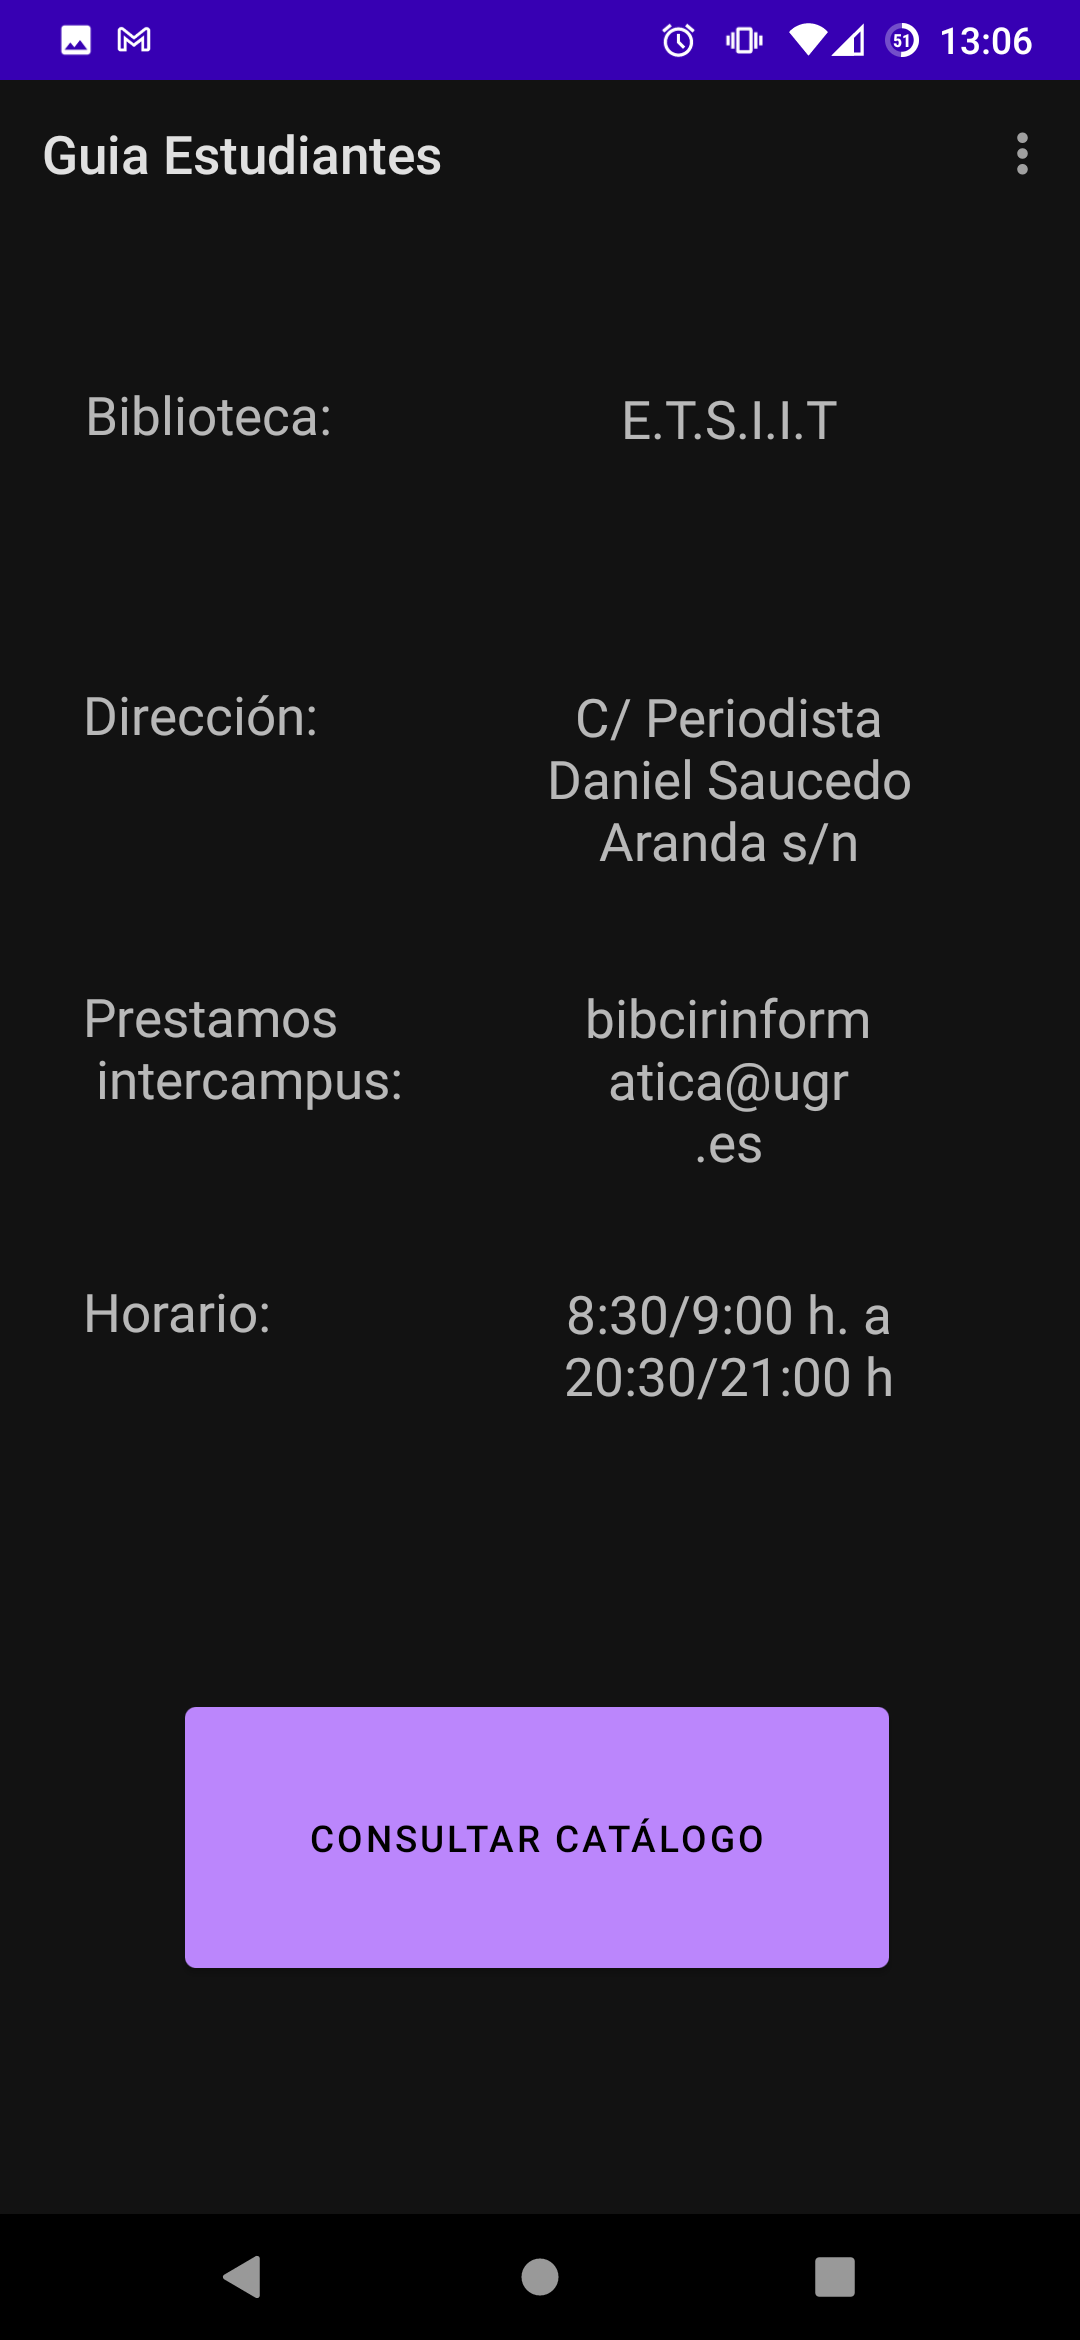
\includegraphics[width=1\linewidth]{biblioteca1.png}
    \caption{Bibliotecas}
    \label{fig:sub-first}
  \end{subfigure}
  \begin{subfigure}{0.5\textwidth}
    \centering
    % include second image
	  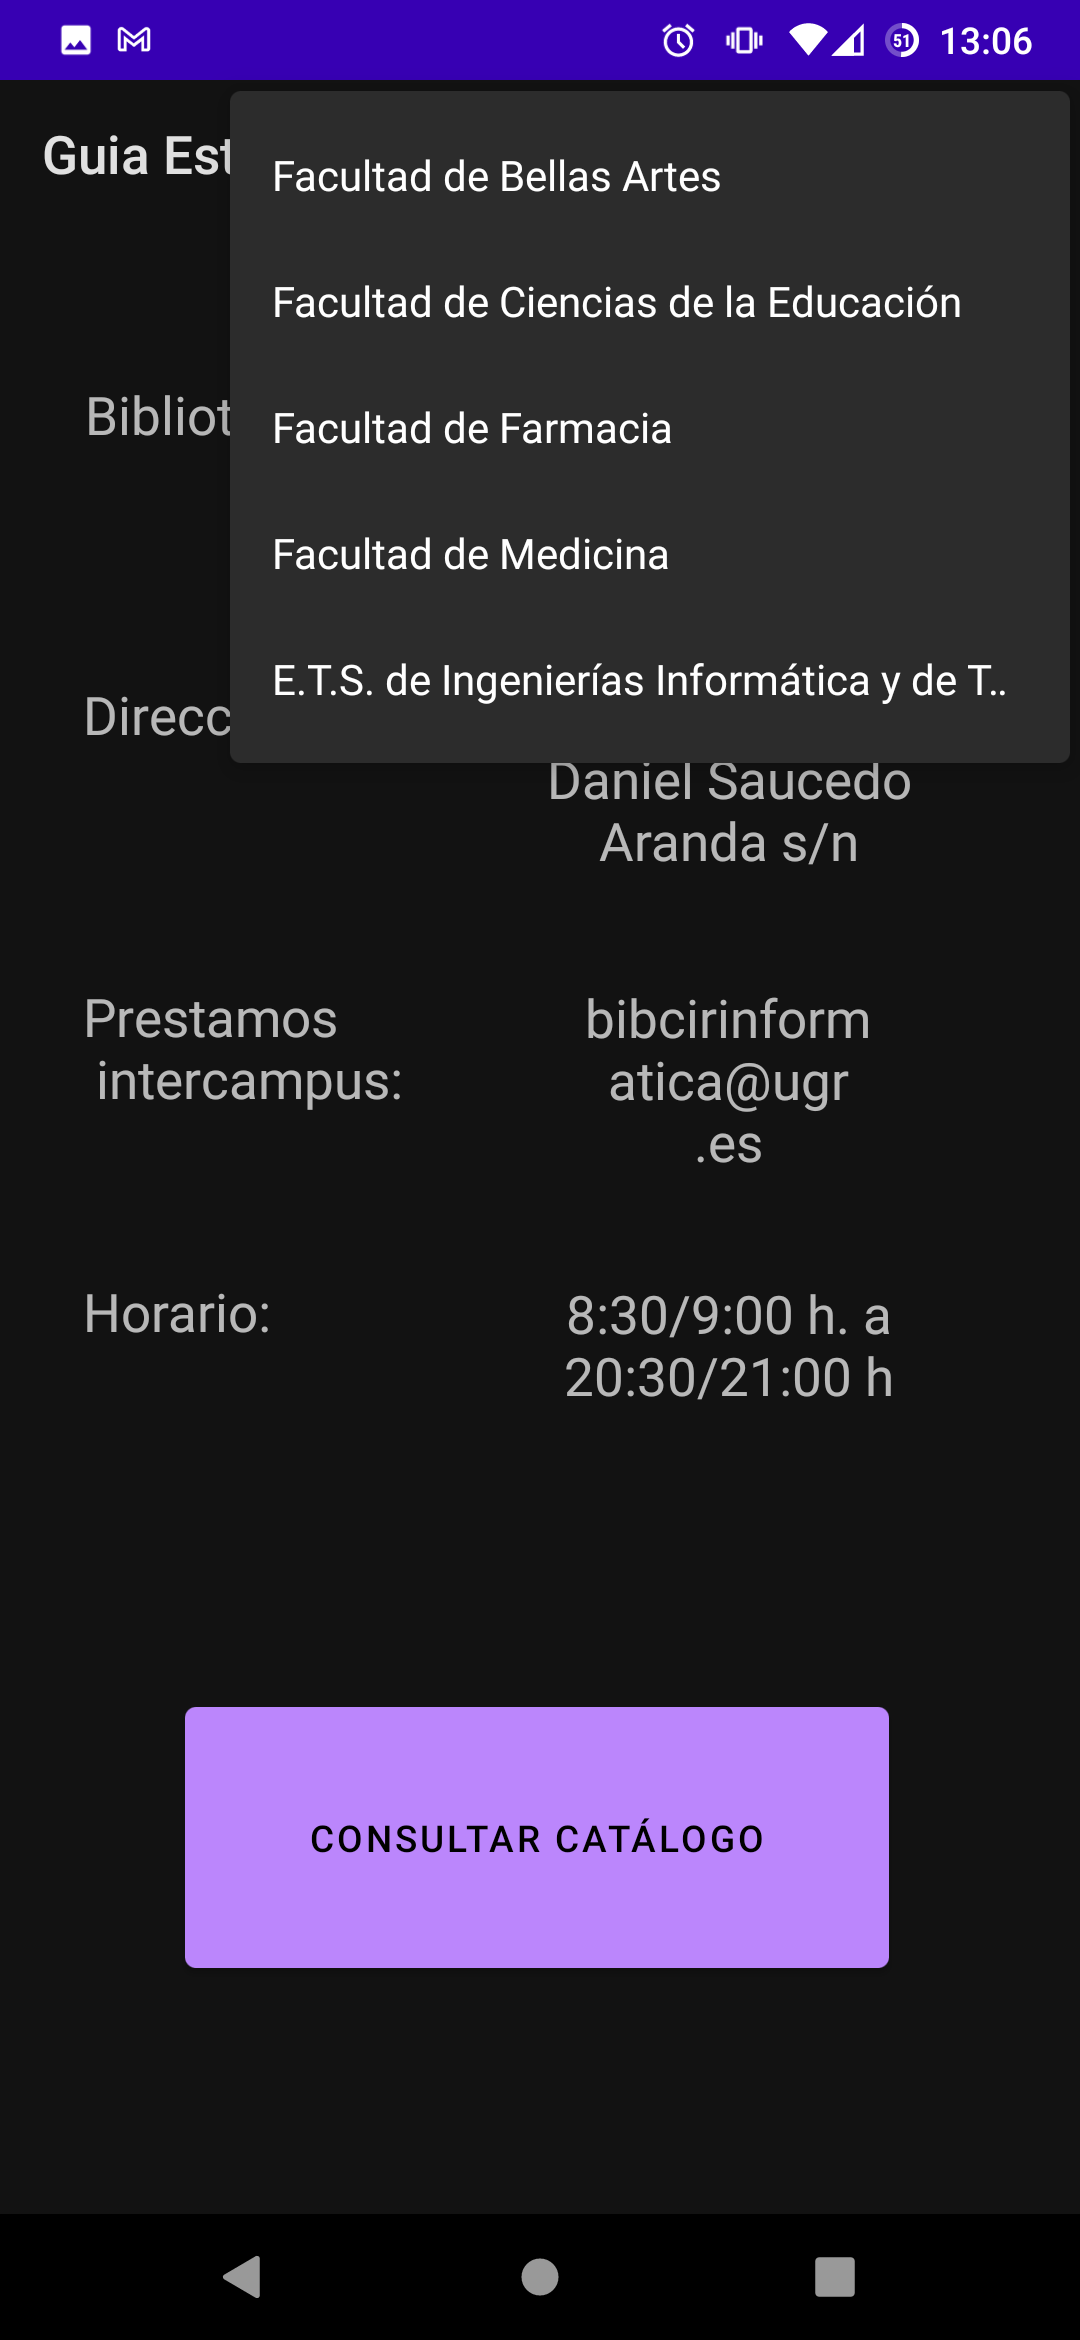
\includegraphics[width=1\linewidth]{biblioteca2.png}
    \caption{Bibliotecas: Menú }
    \label{fig:sub-second}
  \end{subfigure}
\end{figure}





